% http://www2.ual.es/Master-TAII/faq/ % Pinchar en el apartado
% ``Normativa y calendario de TFM'', luego en ``Normativa y Anexos
% Específicos para el TFM'', y descomprimir el archivo, en
% NormativaTFM_MásterTAII.pdf está la normativa. También (en la
% carpeta Anexos) hay otros archivos con las ``plantillas'' para el
% anteproyecto, y el formato de la memoria.

\documentclass[titlepage, 12pt, a4paper, oneside]{article}
\usepackage[utf8]{inputenc}
\usepackage[spanish, es-tabla]{babel}
\usepackage[T1]{fontenc}
\usepackage{hyperref}
\usepackage[numbib]{tocbibind}
\usepackage{tikz}
\usepackage[top=1in, bottom=1.25in, left=1.25in, right=1.25in]{geometry}
\usepackage{xcolor}

\usepackage{fancyhdr}
\pagestyle{fancy}
\fancyhf{}
\rhead{\textit{\color[rgb]{0.0,0.424,0.616}Nombre del estudiante}}
\lhead{}
\rfoot{}
\renewcommand{\headrulewidth}{0pt}

\title{}
\date{}
\renewcommand{\familydefault}{\sfdefault}

\begin{document}
\thispagestyle{empty}
\tikz[remember picture,overlay] \node[opacity=1.0,inner sep=0pt] at (current page.center){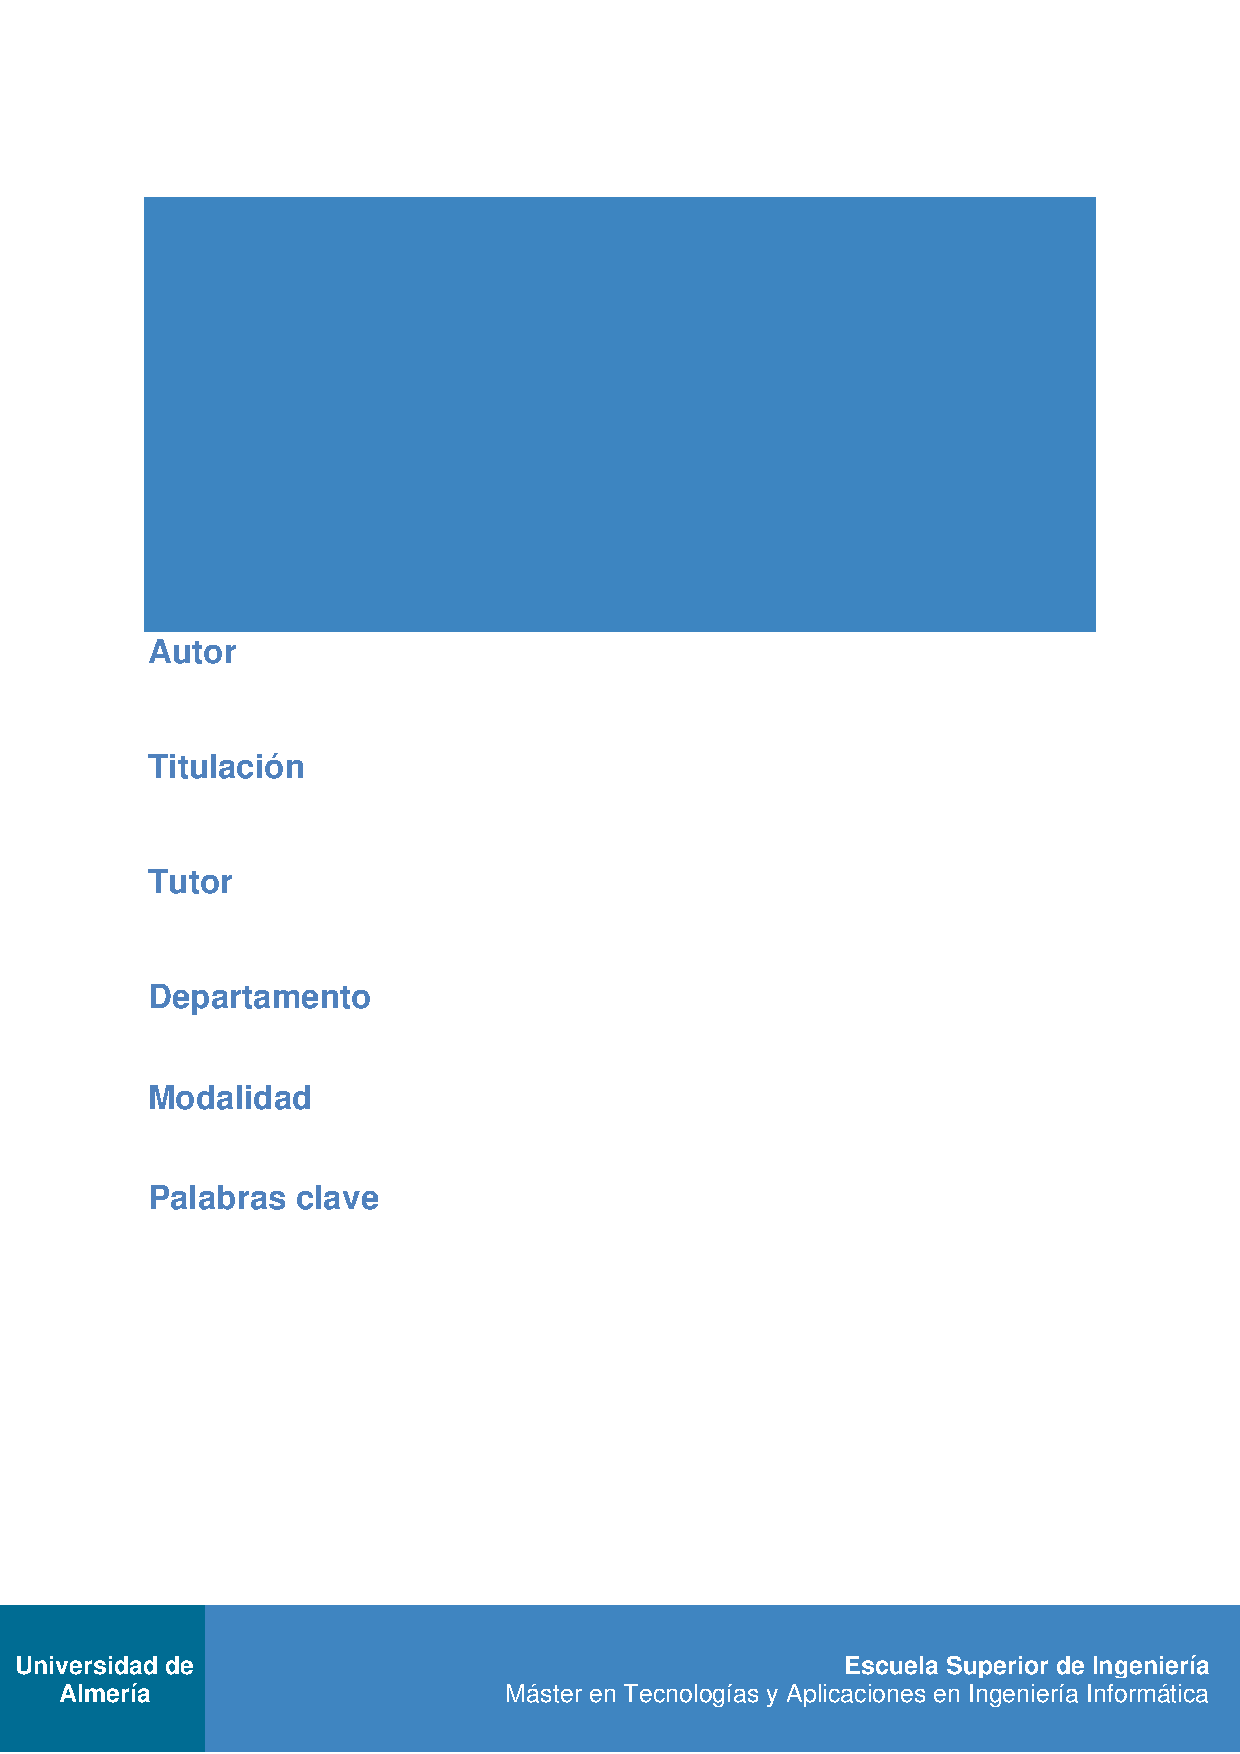
\includegraphics[width=\paperwidth,height=\paperheight]{Plantilla_AnteProyectoTFM-portada}};

\begin{center}
  \vspace{6cm}
  {\color{white} \Huge \textbf{Título del Proyecto}}
\end{center}

\Large

\vspace{-0.2ex}
\begin{tabular}{ll}
  ~~~~~~~~~~~~~~~~~ & Nombre del estudiante
\end{tabular}

\vspace{1.1cm}
\begin{tabular}{ll}
  ~~~~~~~~~~~~~~~~~ & Máster en Tecnologías y Aplicaciones \\
  & en Ingeniería Informática
\end{tabular}

\vspace{0.4cm}
\begin{tabular}{ll}
  ~~~~~~~~~~~~~~~~~ & Vicente González Ruiz
\end{tabular}

\vspace{1.1cm}
\begin{tabular}{ll}
  ~~~~~~~~~~~~~~~~~ & Departamento de Informática
\end{tabular}

\vspace{0.95cm}
\begin{tabular}{ll}
  ~~~~~~~~~~~~~~~~~ & Trabajo Técnico o Trabajo de Investigación
\end{tabular}

\vspace{0.95cm}
\begin{tabular}{ll}
  ~~~~~~~~~~~~~~~~~ & Bla, bla, bla
\end{tabular}

\clearpage

\tikz[remember picture,overlay] \node[opacity=1.0,inner sep=0pt] at (current page.center){
\includegraphics[width=\paperwidth,height=\paperheight]{Plantilla_AnteProyectoTFM-paginas}};

\normalsize

\section{Introducción}
\cite{einstein1922kosmologische}
En esta sección se comentarán las características del problema a resolver, los antecedentes del TFM y la justificación del mismo.

\section{Objetivos y justificación}
En esta sección se comentará el objetivo principal a conseguir en este TFM y los sub-objetivos necesarios para llevarlos a cabo.

\section{Fases de desarrollo}
En esta sección se comentarán las distintas fases en las que se ha dividido el trabajo a realizar.

\section{Materiales y métodos}
En esta sección se comentarán los diferentes materiales o herramientas y métodos o técnicas necesarias para la realización del TFM

\bibliographystyle{plain}
\bibliography{../bibliografia}

\begin{center}
  \textbf{Firmas de los tutores}
\end{center}

\end{document}
